\chapter{Porovnání úspěšnosti metod klasifikace\label{cpt:compare}}% MARK: Porovnání úspěšnosti metod klasifikace
% \note{Shrnutí analýzy $D_\text{SH}$ a $D_\text{D}$ z \cite{remarks}. Experimentální(?) poznatky z \cite{galligan} a soupis vhodných rozsahů pro jednotlivé metody. Výhody $D_\text{N}$.}
Kritickým bodem každého z kritérií je vhodné zvolení hraniční hodnoty $D_\text{max}$\footnote{V této kapitole vynecháváme \citeauthor{radiosurvey}ovu metodu přímého porovnávání elementů dráhy, která se nerozšířila a dostupné zdroje se její úspěšností nezabývají.};
$$
    D(A,B)\le D_\text{max}\text{.}
$$
Každé z $D$-kritérií pracuje s elementy dráhy jinak a nabývá odlišných hodnot, proto je pro jejich správné fungování nezbytné tyto hranice nastavit tak, aby kritéria zachytila co nejvíce členů meteorického roje, ale minimalizovala přítomnost meteoroidů ze sporadického pozadí a nezahrnovala do roje žádné členy jiného roje.

\section{Stanovení hraničních hodnot kritérií}% MARK: Stanovení hraničních hodnot

Autoři jednotlivých kritérií podle svých zkušeností a existujících dat o meteorických rojích nastavili hraniční hodnoty tak, aby byly vyhovující pro jejich účely. Tyto hranice však nebyly vždy plně vyhovující pro obecnější užití těchto kritérií. Například se ukázalo, že je potřeba tuto hraniční hodnotu zvyšovat pro dráhy s vyšší inklinací \cite{galligan}, a některá kritéria nejsou vůbec vhodná pro retrográdní orbity \cite{galligan} ($i>90^\circ$, těleso obíhá proti směru rotace Slunce).

\medskip

Nalezením vhodných hraničních hodnot se ve své práci \cite{galligan} věnoval \citeauthor{galligan}. Ten nejprve identifikoval, že pro meteoroidy obíhající blízko ekliptiky (inklinace blízká $90^\circ$ či $180^\circ$) jsou členy $D$-funkcí obsahující inklinaci velmi malé, a že je tedy nutné hraniční hodnoty měnit v závislosti na inklinaci. Usoudil, že je pro účely $D$-kritéria adekvátní rozdělit orbity do tří kategorií dle inklinace \cite{galligan}:
\begin{enumerate}
    \item \hspace{1cm} $i < 10^\circ$,
    \item \hspace{1cm} $10^\circ \le i < 90^\circ$ a
    \item \hspace{1cm} $i \ge 90^\circ$ (retrográdní orbity).
\end{enumerate}
Pro každý tento interval pak určoval hraniční hodnotu $D_\text{max}$ zvlášť.

\smallskip

Pro určení hodnot zvolil malou množinu reálných meteoroidů se známými drahami a Monte Carlo metodou nasimuloval pro každý z nich několik desítek tisíc perturbovaných meteoroidů, které reprezentovaly roj vzniklý z původního meteoroidu jakožto mateřského tělesa \cite{galligan}. Simulované orbity poté jednotlivými $D$-kritérii porovnával s mateřským tělesem pro postupně se zvyšující hodnotu $D_\text{max}$ a zaznamenával, kolik procent simulovaných meteoroidů kritérium s danou hraniční hodnotou splňovalo. Výsledek tohoto pokusu pro dvě mateřská tělesa ukazují grafy v obrázku \ref{img:performance:recovery}.

\begin{figure}[ht]
    \centering
    \subfigure[denní Sextantidy (prográdní)]{
        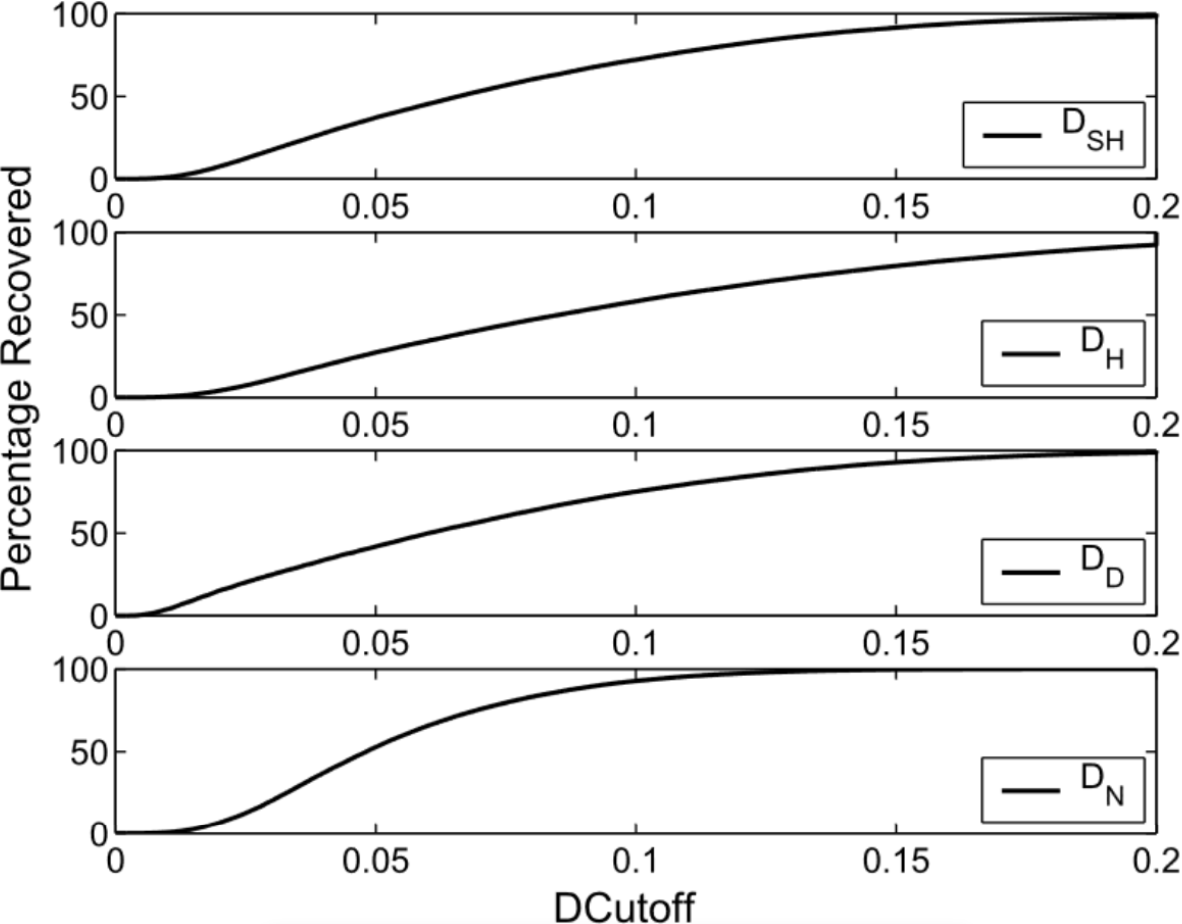
\includegraphics[width=0.45\linewidth]{img/plots/performance-recovery-dsx.png}
        \label{img:performance:recovery:prograde}
    }\hfill
    \subfigure[$\eta$ Aquaridy (retrográdní)]{
        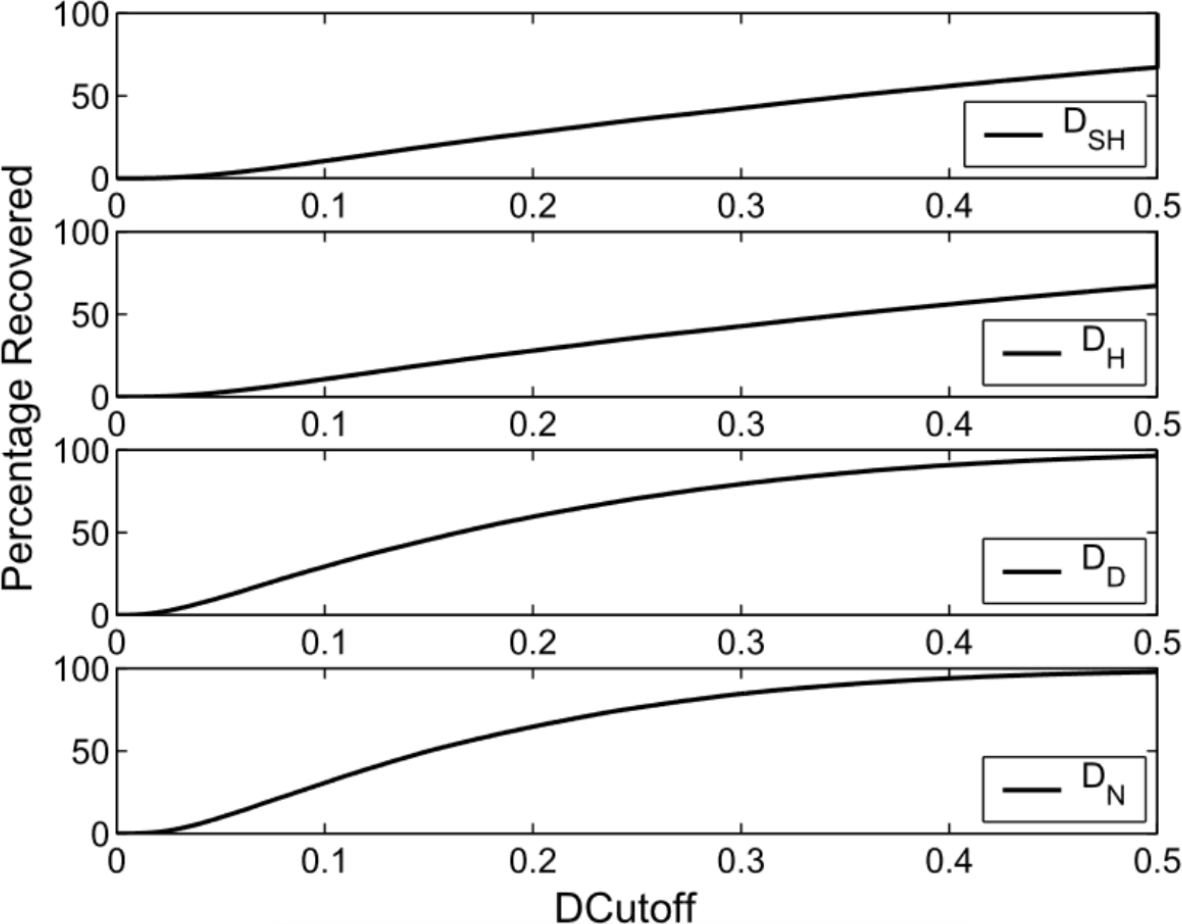
\includegraphics[width=0.45\linewidth]{img/plots/performance-recovery-eaq.png}
        \label{img:performance:recovery:retrograde}
    }
    \caption[Procento simulovaných orbitů splňující $D$-kritéria]{
        Procento simulovaných orbitů splňující jednotlivá kritéria v závislosti na $D_\text{max}$ (zde \textsf{DCutoff})\\
        {\small (zdroj: \cite{galligan})}
    }
    \label{img:performance:recovery}
\end{figure}

\medskip

Ultimátním výsledkem \citeauthor{galligan}ovy práce bylo stanovení hraničních hodnot pro jednotlivá $D$-kritéria. Tyto hodnoty jsou pro každé kritérium rozdělena ještě podle inklinace a podle požadovaného procenta simulovaných meteoroidů splňujících kritérium. Přikládáme je v tabulce \ref{tbl:performance:cutoffs} a hodnoty pro $70\:\%$ splňujících meteoroidů jsme uvedli u jednotlivých kritérií.

\begin{table}[ht]
    \centering
    \caption[Hraniční hodnoty pro jednotlivá $D$-kritéria]{
        Hraniční hodnoty pro jednotlivá $D$-kritéria\\
        {\small (zdroj: \cite{galligan})}
    }
    \begin{tabular}{|l|c|c c c c|}
        \hline
        Inklinace                   & Procento    & $D_\text{SH}$ & $D_\text{D}$ & $D_\text{H}$ & $D_\text{N}$ \\
                                    & splňujících &               &              &              &              \\
        \hline
                                    & $50\:\%$    & $0{,}06$      & $0{,}04$     & $0{,}07$     & $0{,}06$     \\
        $i < 10^\circ$              & $70\:\%$    & $0{,}09$      & $0{,}06$     & $0{,}10$     & $0{,}08$     \\
                                    & $90\:\%$    & $0{,}13$      & $0{,}09$     & $0{,}14$     & $0{,}11$     \\
        \hline
                                    & $50\:\%$    & $0{,}08$      & $0{,}08$     & $0{,}11$     & $0{,}06$     \\
        $10^\circ \le i < 90^\circ$ & $70\:\%$    & $0{,}12$      & $0{,}11$     & $0{,}16$     & $0{,}09$     \\
                                    & $90\:\%$    & $0{,}20$      & $0{,}18$     & $0{,}23$     & $0{,}14$     \\
        \hline
                                    & $50\:\%$    & $0{,}25$      & $0{,}12$     & $0{,}25$     & $0{,}12$     \\
        $i \ge 90^\circ$            & $70\:\%$    & --            & $0{,}18$     & --           & $0{,}17$     \\
                                    & $90\:\%$    & --            & $0{,}28$     & --           & $0{,}26$     \\
        \hline
    \end{tabular}
    \label{tbl:performance:cutoffs}
\end{table}

Kritéria $D_\text{SH}$ a $D_\text{H}$ v tabulce \ref{tbl:performance:cutoffs} neobsahují hodnoty pro retrográdní orbity. Přesahují totiž hodnoty $D$-funkce, ve kterých se již překrývají značně odlišné roje \cite{galligan}. Není proto doporučeno tato kritéria pro retrográdní orbity používat.

\section{Diskuse úspěšnosti kritérií}% MARK: Diskuse úspěšnosti
Od kritérií chceme, aby s co nejnižší hraniční hodnotou $D_\text{max}$ zachytila co nejvíce meteorů patřících do roje (a také minimalizovala přítomnost meteorů ze sporadického pozadí, to však pro účely této diskuse považujme za sekundární). Toto chování nejlépe vykazuje kritérium $D_\text{N}$ v grafu \ref{img:performance:recovery:prograde} dole: V okolí $D_\text{max}=0{,}05$ procento splňujících narůstá velmi rychle a překračuje $50\:\%$ dříve než všechna ostatní kritéria. Graf \ref{img:performance:recovery:retrograde} ukazuje, že se $D_\text{N}$ chová velmi dobře i v retrográdních orbitech. Škála vodorovné osy je zde sice odlišná, hranici $50\:\%$ však stále překračuje jako první a konkurencí mu je pouze \citeauthor{cometassoc}ovo kritérium $D_\text{D}$.

$D_\text{N}$ je také velmi stabilní v hraničních hodnotách pro různé inklinace; jak ukazuje tabulka \ref{tbl:performance:cutoffs}, mezi jednotlivými kategoriemi inklinací se jeho hraniční hodnota mění nejpomaleji. Dobře zvládá také retrográdní orbity.

\smallskip

Takto "`na papíře"' se tedy jako nejúspěšnější kritérium jeví $D_\text{N}$, které navrhli \citeauthor{newapproach}. Při jeho implementaci a testování v programovém nástroji vyvíjeném v rámci praktické části této práce (viz kapitola \ref{cpt:practical}) jsme ale objevili pár jeho slabých míst.

Prvním z nich je skutečnost, že toto kritérium funguje pouze na eliptických orbitech: Vyžaduje totiž délku velké poloosy $a$, která v parabolických drahách jde do nekonečna (narozdíl od ostatních kritérií, která využívají vzdálenost perihélia $q$ dobře definovanou pro všechny kuželosečky). Pro hyperbolické dráhy pak selhává výpočet geocentrické rychlosti \eqref{eqn:geocentric:u}, kde se odmocňuje záporné číslo.

Druhým jeho slabým místem je zjevná přílišná "`svolnost"' v přijímání meteorů do rojů, kterou jsme pozorovali při testování programu. Na datech, která nám pro účely vývoje byla poskytnuta, ostatní kritéria identifikovala příslušnost k jednomu až dvěma meteorickým rojům, ovšem $D_\text{N}$ dával příslušnost až k $>5$ rojům. Ačkoliv uznáváme, že tato vlastnost může být přínosná k identifikaci nových meteorických rojů, při přiřazování do stávajících rojů spíše komplikuje práci vnášením nejednoznačnosti.

\smallskip

Při našem testování na dostupných datech dávaly nejkonzistentnější výsledky kritéria $D_\text{SH}$ a $D_\text{D}$. Až na výjimečné případy se shodovaly v přiřazení meteoru do meteorického roje a i podle grafů v obrázků \ref{img:performance:recovery} vykazují dobrou úspěšnost. Kritérium $D_\text{SH}$ sice nefunguje dobře v retrográdních orbitech, tam jej ale dobře zastupuje $D_\text{D}$.

\medskip

Následující ukázka výstupu,\footnote{Výstup byl zarovnán pro lepší čitelnost.} zatím bez jakéhokoliv hlubšího vysvětlení, ilustruje diskutovanou "`svolnost"' kritéria $D_\text{N}$ (a v menší míře i konzistentnost $D_\text{SH}$ a $D_\text{D}$):
\begin{Verbatim}[commandchars=\\\{\},gobble=4,formatcom=\tiny,codes={\catcode`$=3\catcode`^=7},frame=lines]
    ***** Result 10C12041 *****
    \eCheck  [GEM] Geminids   D(sh)=0.050 (cutoff 0.09)  D(d)=0.071 (cutoff 0.09)  D(h)=0.083 (cutoff 0.1)  D(n)=0.019 (cutoff 0.08)
                        D(sh)=0.045 (cutoff 0.09)  D(d)=0.071 (cutoff 0.09)  D(h)=0.081 (cutoff 0.1)  D(n)=0.021 (cutoff 0.08)
                        D(sh)=0.050 (cutoff 0.09)  D(d)=0.071 (cutoff 0.09)  D(h)=0.083 (cutoff 0.1)  D(n)=0.019 (cutoff 0.08)
                        D(sh)=0.041 (cutoff 0.09)  D(d)=0.070 (cutoff 0.09)  D(h)=0.078 (cutoff 0.1)  D(n)=0.022 (cutoff 0.08)
                        D(sh)=0.047 (cutoff 0.09)  D(n)=0.042 (cutoff 0.08)
    \eCheck  [XLI] April $\chi$ Librids   D(n)=0.023 (cutoff 0.08)
    \eCheck  [SAR] September $\mu$ Arietids   D(n)=0.025 (cutoff 0.08)
    \eCheck  [THA] November $\theta$ Aurigids   D(n)=0.036 (cutoff 0.08)  D(n)=0.068 (cutoff 0.08)
    \eCheck  [DLT] Daytime $\lambda$ Taurids   D(n)=0.056 (cutoff 0.08)
    \eCheck  [OCE] Southern Daytime $\omega$ Cetids   D(n)=0.068 (cutoff 0.08)
    \eCheck  [SZC] Southern June Aquilids   D(n)=0.069 (cutoff 0.08)
    \eCheck  [AAL] April $\alpha$ Librids   D(n)=0.070 (cutoff 0.08)
    \eCheck  [DRG] December $\rho$ Geminids   D(d)=0.080 (cutoff 0.09)
    \eCheck  [IAR] November $\iota$ Aurigids   D(n)=0.074 (cutoff 0.08)
    \eCross  [ARI] Daytime Arietids   D(n)=0.080 (cutoff 0.08)
    \eCross  [SAR] September $\mu$ Arietids   D(n)=0.082 (cutoff 0.08)
    \eCross  [DSX] Daytime Sextantids   D(n)=0.088 (cutoff 0.08)
\end{Verbatim}
Srovnávaný meteor v této ukázce zjevně spadal do Geminid, což zde dle prvního výsledku odhalila všechna kritéria. Kritérium $D_\text{N}$ (v ukázce \texttt{D(n)}) zde však splnilo i dalších devět rojů, do nichž je příslušnost daného meteoru spíše pochybná. Poslední tři řádky ukazují tři nejlepší zamítnuté příslušnosti, které jsou zde kompletně zaplněny výsledky kritéria $D_\text{N}$. 

\medskip

Smutným případem je bohužel kritérium $D_\text{H}$, které přes své optimální matematické vlastnosti dávalo nejhorší výsledky jak podle \citeauthor{galligan}ových pokusů, tak při našem testování. Grafy v obrázku \ref{img:performance:recovery} ukazují, že je jeho úspěšnost nejhorší ze všech, a při testování na nám dostupných datech se chovalo spíše jako striktnější varianta $D_\text{SH}$